\documentclass[a4paper, 10pt]{article}
\usepackage{amsmath}
\usepackage{caption}
\usepackage{fancyhdr}
\usepackage{float}
\usepackage[a4paper, left=1in, right=1in, top=1in, bottom=1in]{geometry}
\usepackage{graphicx}
\usepackage{minted}
\usepackage{multirow}
\usepackage{physics}
\usepackage{siunitx}
\usepackage{tikz}
\AtBeginDocument{\RenewCommandCopy\qty\SI}
\usepackage{xcolor} % Required for defining custom colors
\captionsetup{justification=centering, skip=10pt} % skip=10pt adds the gap
% --- Modern Dark Monokai Setup ---
\usemintedstyle{monokai}
\definecolor{monokaibg}{HTML}{272822} % The classic Monokai background
\definecolor{linegray}{HTML}{49483E} % Darker grey for line numbers

\lhead{}
\rhead{ECE 456 Problem Set 2}
\headheight 15pt
\pagestyle{fancy}

\newcommand{\ham}{\hat{\mathcal{H}}}

\begin{document}

\begin{titlepage}
    \vspace*{\fill}
    \begin{center}
        \Huge\textbf{ECE 456 Problem Set 2:\\}
        The Schrödinger Equation \\
        \vspace{1cm}
        \Large Omar Mahmoud, Nasif Qadri\\
        \vspace{0.5cm}
        \normalsize \today
    \end{center}
    \vspace*{\fill}
\end{titlepage}

\section{Numerical Solution for the Particle in a Box}

\subsection{Numerical Implementation and Eigenvalue Extraction}
% 1a
Consider the problem of a particle in an escape-proof box. The code in \verb|1a.py| was used to find the eigenvectors and eigenvalues of the correspodning matrix equation $[\ham] \{\phi\} = E \{\phi\}$. The lattice points are defined from $n = 1$ to $n = N$, with $N = 100$ and lattice constant $a = \qty{1}{\AA}$. \\

\noindent When ran, \verb|1a.py| generated the plots found in Figures \ref{fig:1a_probdensity} and \ref{fig:1a_eigenvalues}.

\begin{figure}[H]
    \centering
    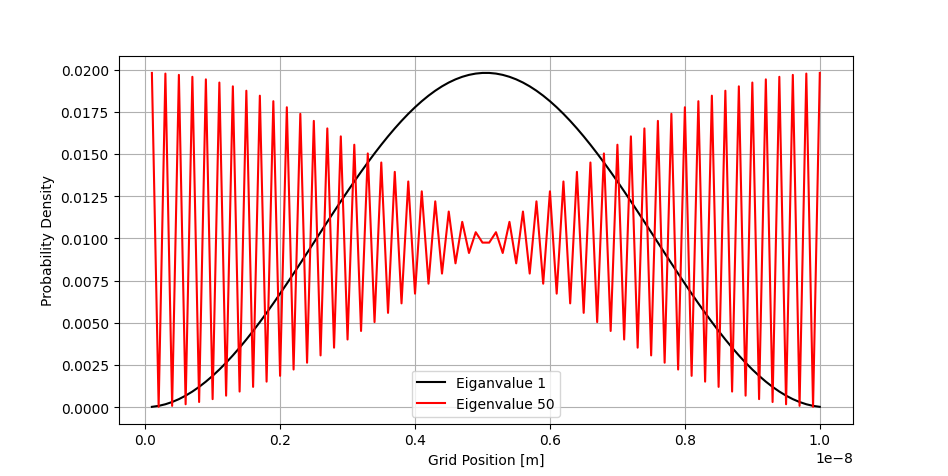
\includegraphics[width=0.7\textwidth]{imgs/1a_probdensity.png}
    \caption{Position-probability densities from the numerical wave functions $\{\phi\}$ for eigenvalue numbers $1$ and $50$.}
    \label{fig:1a_probdensity}
\end{figure}

\begin{figure}[H]
    \centering
    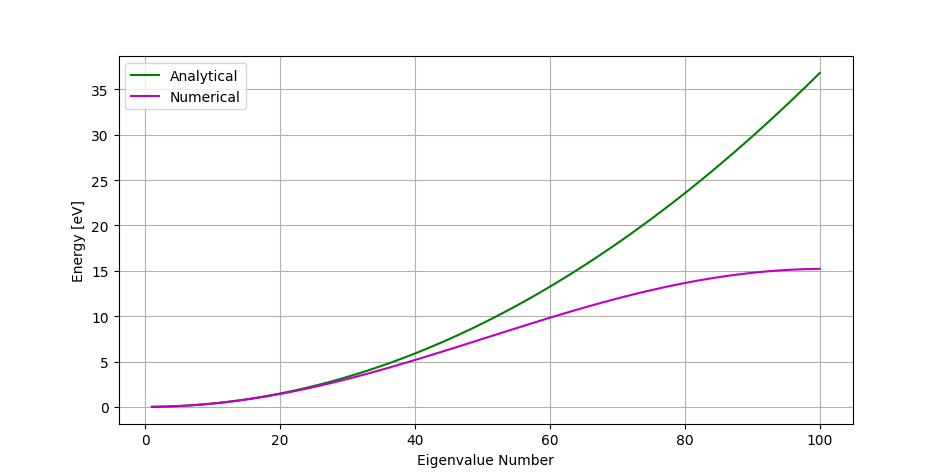
\includegraphics[width=0.7\textwidth]{imgs/1a_eigenvalues.png}
    \caption{The 100 eigenvalues that resulted from the numerical and analytical solutions.}
    \label{fig:1a_eigenvalues}
\end{figure}

% 1b
\subsection{Normalization of Analytical and Numerical Representations}

% (i)
\subsubsection{Normalization of the Analytical Wave Function}
\noindent The analytical solution can be written as
\begin{equation}
    \phi(x) = A \sin \left( \frac{n \pi}{L} x \right)
\end{equation}
where $A$ is a constant, and where the box extends from $x = 0$ to $x = L$. Normalization requires
\begin{equation} \label{eq:1b_analytical_sol}
    \int_{0}^{L} |\phi(x)|^2 \dd{x} = 1
\end{equation}
The value of $A$ required to properly normalize the analytical wave function can be found by
\begin{align*}
    &\int^L_0 |\phi(x)|^2\dd{x} = 1 \\
    &\int^{L}_{0} \left| A \sin \left( \frac{n \pi x}{L} \right) \right|^2 \dd{x} = 1 \\
    &\int^{L}_{0} A^2 \sin^2 \left( \frac{n \pi x}{L} \right) \dd{x} = 1 \\
    &A^2 \left[ \frac{1}{2}x - \frac{L}{4 n \pi}\sin \left( \frac{2n \pi x}{L} \right) \right]^L_0 = 1 \\
    &A^2 \left[ \frac{x}{2} - \frac{L}{4n \pi}\sin \left( \frac{2n \pi x}{L} \right) \right]^L_0 = 1 \\
    &A^2 \left[ \left( \frac{L}{2} - \frac{L}{4n \pi}\sin(2n\pi) \right) - \left( 0 - \frac{L}{4n \pi}\sin(0) \right) \right] = 1 \\
    &A^2 \left( \frac{L}{2} \right) = 1 \\
    &A^2 = \frac{2}{L} \\
    &\boxed{ A = \sqrt{\frac{2}{L}} }
\end{align*}

% (ii)
\subsubsection{Numerical Normalization and the Continuum Limit}
\noindent For sufficiently small values of the lattice constant $a$, it is reasonable to assume that the $\ell$th component of the numerical eigenvector $\{\phi\}$ will follow a functional form that is consistent with (\ref{eq:1b_analytical_sol}), and will be given, for example, by
\begin{equation}
    \phi_{\ell} = B \sin \left( \frac{n \pi}{L} x_{\ell} \right)
\end{equation}
where $B$ is a normalization constant and $x_{\ell} = a\ell$ is the $\ell$th lattice point. If the numerical eigenvectors are normalized according to the equation
\begin{equation}
    \sum_{\ell=1}^{N} |\phi_{\ell}|^2 = 1
\end{equation}
the expected value of $B$ in the limit that $a \to 0$ can be found by
\begin{align*}
    &\sum^N_{\ell=1} \left| \phi_{\ell} \right|^2 = 1 \\
    &a\sum^N_{\ell=1} \left| \phi_{\ell} \right|^2 = a \\
    &a\sum^N_{\ell=1} \left| B \sin \left( \frac{n \pi}{L} x_\ell \right) \right|^2 = a \\
    \intertext{As $a \rightarrow 0$ the total number of lattices $N \rightarrow \infty$ (Riemann sum), therefore this becomes:}
    &\int_0^L B^2 \sin^2\left(\frac{n\pi x}{L}\right) \dd{x} = a \\
    &B^2 \left( \frac{L}{2} \right) = a \\
    &B^2 = \frac{2a}{L} \\
    &\boxed{B = \sqrt{\frac{2a}{L}}}
\end{align*}

% 1c
\subsection{Investigation of Numerical Eigenvalue Deviation}

% (i)
\subsubsection{Derivation of the Discrete Dispersion Relation}
\noindent The discretized time-independent Schrödinger equation is given by:
\begin{equation*}
    -t_{0}\phi_{\ell-1} + (2t_{0} + U_{\ell})\phi_{\ell} - t_{0}\phi_{\ell+1} = E\phi_{\ell}
\end{equation*}
For a particle in a box, the potential inside is zero ($U_{\ell} = 0$). We assume the ansatz $\phi_{\ell} = B \sin(k x_{\ell}) = B \sin(k a \ell)$ with $k = \frac{n\pi}{L}$. Rearranging the difference equation:
\begin{align*}
    -t_{0}(\phi_{\ell-1} + \phi_{\ell+1}) + 2t_{0}\phi_{\ell} &= E\phi_{\ell}
\end{align*}
Using the trigonometric addition and subtraction identities:
\begin{align*}
    \phi_{\ell-1} &= B \sin(ka(\ell-1)) = B \left[ \sin(ka\ell)\cos(ka) - \cos(ka\ell)\sin(ka) \right] \\
    \phi_{\ell+1} &= B \sin(ka(\ell+1)) = B \left[ \sin(ka\ell)\cos(ka) + \cos(ka\ell)\sin(ka) \right]
\end{align*}
Summing these terms cancels the cosine-sine terms:
\begin{align*}
    \phi_{\ell-1} + \phi_{\ell+1} &= 2B \sin(ka\ell)\cos(ka) \\
    &= 2\phi_{\ell} \cos(ka)
\end{align*}
Substituting this back into the rearranged difference equation:
\begin{align*}
    -t_{0}(2\phi_{\ell} \cos(ka)) + 2t_{0}\phi_{\ell} &= E\phi_{\ell} \\
    2t_{0}\phi_{\ell} - 2t_{0}\phi_{\ell} \cos(ka) &= E\phi_{\ell} \\
    2t_{0}\phi_{\ell} (1 - \cos(ka)) &= E\phi_{\ell}
\end{align*}
Dividing both sides by $\phi_{\ell}$ and substituting $k = \frac{n\pi}{L}$:
\begin{equation}\label{eq:1c_energy}
\boxed{
    E = 2t_{0} \left[ 1 - \cos\left( \frac{n\pi a}{L} \right) \right]
}
\end{equation}

% (ii)
\subsubsection{Validation of Results}
\begin{figure}[H]
    \centering
    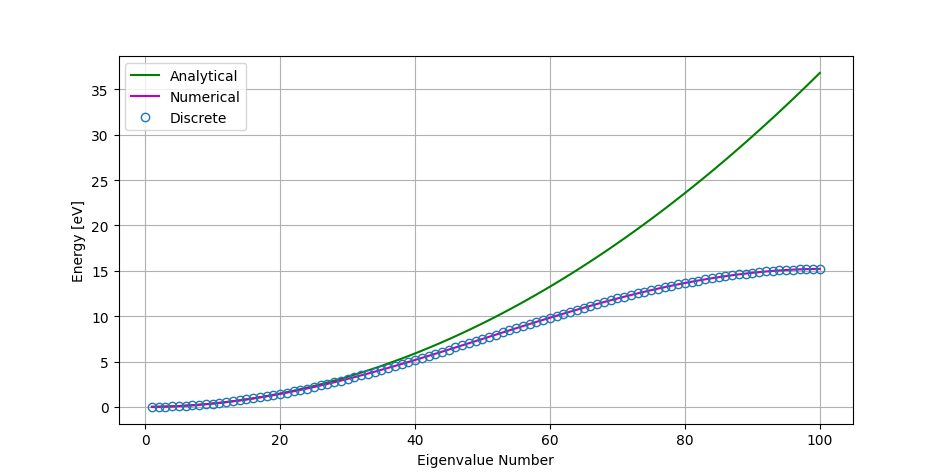
\includegraphics[width=0.7\textwidth]{imgs/1c.png}
    \caption{Comparison of the analytical energy eigenvalues (solid line), the numerical eigenvalues obtained via the finite difference method (x's), and the expected discrete eigenvalues derived in Equation \ref{eq:1c_energy} (circles).}
    \label{fig:1c_eigenvalue}
\end{figure}

\noindent The plot demonstrates that the discrete energy expression derived in Equation \ref{eq:1c_energy} matches the numerical eigenvalues (represented by the black x's) perfectly.\\

\noindent This confirms that the deviation of the numerical results from the analytical prediction ($E \propto n^2$) at higher energy levels ($n \ge 50$) is a predictable consequence of the discrete lattice. The finite difference method only approximates the continuous relation when $n$ is small (when the wavelength is large compared to the lattice spacing $a$). \\

% (iii)
\subsubsection{Small-Angle Approximation}
\noindent For small angles $\theta$, the cosine function can be approximated by the Taylor series expansion:
\begin{equation*}
    \cos\theta \approx 1 - \frac{\theta^2}{2}
\end{equation*}
\noindent Applying this to Equation \ref{eq:1c_energy} where $\theta = \frac{n\pi a}{L}$:
\begin{align*}
    E &= 2t_0 \left[ 1 - \cos\left(\frac{n\pi a}{L}\right) \right] \\
    &\approx 2t_0 \left[ 1 - \left( 1 - \frac{1}{2}\left(\frac{n\pi a}{L}\right)^2 \right) \right] \\
    &= 2t_0 \left[ \frac{1}{2}\frac{n^2 \pi^2 a^2}{L^2} \right] \\
    &= t_0 \frac{n^2 \pi^2 a^2}{L^2}
    \intertext{Substituting $t_0 = \frac{\hbar^2}{2ma^2}$:}
    E &\approx \left( \frac{\hbar^2}{2ma^2} \right) \frac{n^2 \pi^2 a^2}{L^2} \\
    &= \frac{\hbar^2 \pi^2 n^2}{2mL^2}
\end{align*}

\noindent The result is consistent with the plot in Figure \ref{fig:1c_eigenvalue}. For small values of $n$ (where the angle $\frac{n\pi a}{L}$ is small), the discrete energy expression reduces exactly to the analytical eigenvalue expression $E = \frac{\hbar^2 \pi^2 n^2}{2mL^2}$. This explains why the numerical and analytical results overlap at low energy levels.\\

% (iv)
\subsubsection{Grid Refinement and Resolution of Sampling Errors}
\noindent By reducing the lattice spacing $a$ by a factor of 10 and increasing $N$ to 1000, the numerical eigenvalues now match the analytical results almost perfectly up to $n=100$. The deviation seen in Figure \ref{fig:1a_eigenvalues} for $n \ge 50$ has vanished. This is because the finer grid provides a better sampling rate, keeping the argument of the cosine in the discrete expression, $\frac{n\pi a}{L}$, small enough that the approximation $\cos(x) \approx 1 - x^2/2$ remains valid for a larger range of $n$.\\

% 1d
\subsection{Periodic Boundary Conditions}

% (i)
\subsubsection{TITLE HERE}
The code in \verb|1d.py| is a modified version of \verb|1a.py| changed to implement periodic boundary conditions. Running \verb|1d.py| to get the eigenvalue numbers 4 and 5 produced the output:
% (ii)
\begin{verbatim}
Eigenvalue 4: 0.060023108288934125 eV
Eigenvalue 5: 0.06002310828893526 eV
\end{verbatim}

\noindent The energy for eigenvalue numbers 4 and 5 is degenerate because both eigenvalues correspond to nearly identical energies. This shows that each energy level (above the ground state) has two distinct wavefunctions (states) associated with it.

% (iii)
\noindent The eigenvalue numbers 1 through 5 can be produced by the same code:
\begin{verbatim}
Eigenvalue 1: -1.431884637890359e-15 eV
Eigenvalue 2: 0.0150205969306892 eV
Eigenvalue 3: 0.015020596930693126 eV
Eigenvalue 4: 0.060023108288934125 eV
Eigenvalue 5: 0.06002310828893526 eV
\end{verbatim}
\begin{figure}[H]
    \centering
    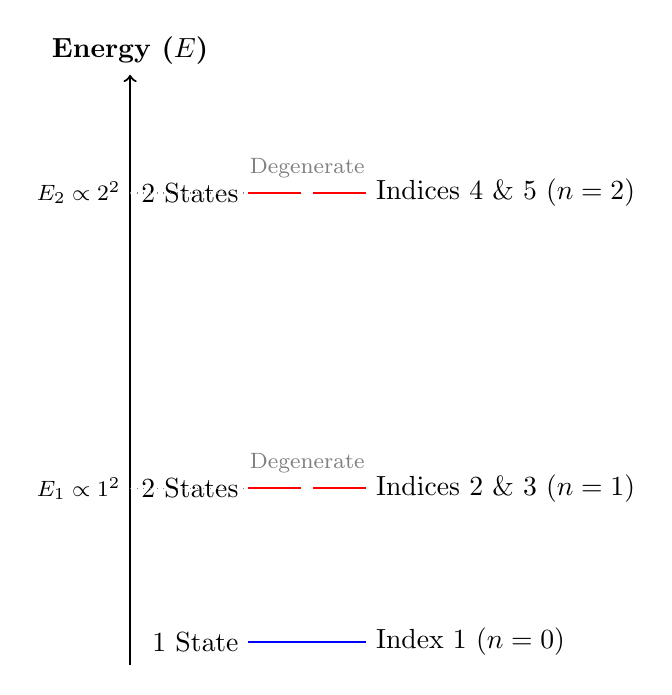
\begin{tikzpicture}[scale=1.5]
        % --- Axis ---
        \draw[->, thick] (-1, 0) -- (-1, 5) node[above] {\textbf{Energy ($E$)}};

        % --- Energy Levels ---

        % Level n=0 (Numerical Index 1)
        % Single state at E ~ 0
        \draw[thick, blue] (0, 0.2) -- (1, 0.2);
        \node[right] at (1, 0.2) {Index 1 ($n=0$)};
        \node[left] at (0, 0.2) {1 State};

        % Level n=1 (Numerical Indices 2 & 3)
        % Degenerate pair (2 states) at E_1
        % Arbitrary height of 1.0 unit
        \draw[thick, red] (0, 1.5) -- (0.45, 1.5);
        \draw[thick, red] (0.55, 1.5) -- (1, 1.5);
        \node[right] at (1, 1.5) {Indices 2 \& 3 ($n=1$)};
        \node[left] at (0, 1.5) {2 States};
        \node[above, font=\footnotesize, gray] at (0.5, 1.55) {Degenerate};

        % Level n=2 (Numerical Indices 4 & 5)
        % Degenerate pair (2 states) at E_2 = 4 * E_1
        % Height should be 4x the distance of the first level (relative to ground)
        % Placing at 4.0 units to show quadratic scaling (1^2 vs 2^2)
        \draw[thick, red] (0, 4.0) -- (0.45, 4.0);
        \draw[thick, red] (0.55, 4.0) -- (1, 4.0);
        \node[right] at (1, 4.0) {Indices 4 \& 5 ($n=2$)};
        \node[left] at (0, 4.0) {2 States};
        \node[above, font=\footnotesize, gray] at (0.5, 4.05) {Degenerate};

        % --- Dashed guidelines for quadratic spacing ---
        \draw[dotted, gray] (-1, 1.5) -- (0, 1.5);
        \node[left, font=\footnotesize] at (-1, 1.5) {$E_1 \propto 1^2$};

        \draw[dotted, gray] (-1, 4.0) -- (0, 4.0);
        \node[left, font=\footnotesize] at (-1, 4.0) {$E_2 \propto 2^2$};

    \end{tikzpicture}
    \caption{Energy-level diagram for a particle in a ring (periodic boundary conditions). Note the single ground state (Index 1) followed by pairs of degenerate states (Indices 2-3, 4-5).}
    \label{fig:ring_energy_levels}
\end{figure}

% (iii)
\subsubsection{Comparison with Analytical Results}
The analytical eigenvalues for a particle in a ring are given by the equation:
\begin{equation}
    E_{analytical} = \frac{2\hbar^2 \pi^2 n^2}{mL^2}
\end{equation}
where $n$ is analytical eigenvalue number. The mapping between the numerical eigenvalue index and the analytical quantum number $n$ is as follows:
\begin{itemize}
    \item Index 1 corresponds to $n=0$.
    \item Indices 2 and 3 correspond to $n=1$.
    \item Indices 4 and 5 correspond to $n=2$.
\end{itemize}

\noindent The comparison between the analytical values and the numerical results is summarized in Table \ref{tab:ring_energies}.

\begin{table}[H]
    \centering
    \caption{Comparison of numerical and analytical eigenvalues for the particle in a ring}
    \label{tab:ring_energies}
    \renewcommand{\arraystretch}{1.2}
    \begin{tabular}{|c|c|c|c|c|}
        \hline
        \textbf{Index} & \textbf{Numerical $E$ [eV]} & \textbf{Analytical $E$ [eV]} & \textbf{Ring $n$} & \textbf{Degeneracy} \\
        \hline
        1 & 0.0000 & 0.0000 & 0 & Non-Degenerate \\
        \hline
        2 & 0.0148 & 0.0149 & 1 & \multirow{2}{*}{Degenerate} \\
        3 & 0.0148 & 0.0149 & 1 & \\
        \hline
        4 & 0.0591 & 0.0596 & 2 & \multirow{2}{*}{Degenerate} \\
        5 & 0.0591 & 0.0596 & 2 & \\
        \hline
    \end{tabular}
\end{table}

\noindent The energies for indices 2 and 3 are virtually identical, as are the energies for indices 4 and 5, confirming the degeneracy expected for a particle in a ring. Small discrepancies between numerical and analytical values can be chalked up to the finite lattice spacing $a$. Therefore, the numerical results are consistent with the analytical predictions.

\section{Radial Equation for the Hydrogen Atom}
The radial part of the solution of the Schrödinger equation for the hydrogen atom can be written in terms of a function $f(r)$ where $|f(r)|^2 \dd{r}$ represents the probability of finding the electron in the volume between $r$ and $r + \dd{r}$, where the nucleus is at the origin $r = 0$. Given that $f(r)$ is govered by the radial Schrödinger equation,
\begin{equation}\label{eq:radial_schro}
    \left[ \frac{-\hbar^2}{2m} \frac{d^2}{dr^2} - \frac{q^2}{4\pi\epsilon_0 r} + \frac{l_o(l_o + 1)\hbar^2}{2mr^2} \right] f(r) = Ef(r)
\end{equation}
where $\epsilon_0 = 8.854 \times 10^{-12}\,\unit{\farad\per\meter}$.

% 2a
% 2b
\subsection{Defining the Hamiltonian Matrix}
If Equation \ref{eq:radial_schro} is rewritten in the form
\begin{equation}
	\ham f(r) = E f(r)
\end{equation}
with
\begin{equation}
	\ham \equiv \left[ \frac{-\hbar^2}{2m} \frac{d^2}{dr^2} - \frac{q^2}{4\pi\epsilon_0 r} + \frac{l_o(l_o + 1)\hbar^2}{2mr^2} \right]
\end{equation}
and boundary conditions are such that $f(r) = 0$ at the endpoints of the discretized space, $[\ham]$ would be defined as
\begin{equation}
[\hat{H}] =
\begin{bmatrix}
2t_0 + U_1 & -t_0 & 0 & \dots & 0 \\
-t_0 & 2t_0 + U_2 & -t_0 & \dots & 0 \\
0 & -t_0 & 2t_0 + U_3 & \dots & 0 \\
\vdots & \vdots & \vdots & \ddots & \vdots \\
0 & 0 & 0 & \dots & 2t_0 + U_N
\end{bmatrix}
\end{equation}
where $U_l$ and $t_0$ are defined as
\begin{equation}
    U_l = -\frac{q^2}{4\pi\epsilon_0 r_n} + \frac{l_0(l_0 + 1)\hbar^2}{2mr_n^2}
\end{equation}
\begin{equation}
    t_0 = \frac{\hbar^2}{2m(\Delta r)^2}
\end{equation}

% 2d
\noindent The code in \verb|1a.py| was modified to what is seen in \verb|2c.py|. \verb|2c.py| was used to produce the plots for the first two eigenvectors, corresponding to the 1s and 2s energy states, as seen in Figures [ADD REF HERE].

\begin{verbatim}
Eigenvalue 1: -13.497781923462465 eV
Eigenvalue 2: -3.396072886508772 eV
\end{verbatim}

% 2d

\section{Appendix}

\begin{listing}[H]
    \caption{Code in 1a.py used to generate Figures \ref{fig:1a_probdensity} and \ref{fig:1a_eigenvalues}.}
    \label{lst:code_1a}
    \inputminted[
        bgcolor=monokaibg,
        frame=leftline,
        rulecolor=\color{linegray}, % Added \color{} command
        framesep=3mm,
        baselinestretch=1.1,
        linenos,
        numbersep=5pt,
        fontsize=\footnotesize,
        breaklines,
    ]{python}{code/1a.py}
\end{listing}

\begin{listing}[H]
    \caption{Code in 1d.py used to generate Figures.}
    \inputminted[
        bgcolor=monokaibg,
        frame=leftline,        % Adds a subtle vertical bar on the left
        rulecolor=linegray,
        framesep=3mm,
        baselinestretch=1.1,
        linenos,
        numbersep=5pt,
        fontsize=\footnotesize,
        breaklines,            % Wraps long lines automatically
    ]{python}{code/1d.py}
\end{listing}
\end{document}
